\documentclass[11pt, letterpaper]{article}
\setlength{\parindent}{0in}
\setlength{\textheight}{8.7in}
\setlength{\textwidth}{6.8in}
\setlength{\oddsidemargin}{-0.3in}
\setlength{\evensidemargin}{0.0in}
\addtolength{\topmargin}{-1in}
\setlength{\parskip}{0.1in}

\usepackage{amsmath, amsfonts, color}
\usepackage{bm}
\usepackage{enumerate}
\usepackage{graphicx}
\newcommand*{\justifyheading}{\raggedleft}


\renewcommand{\baselinestretch}{1.0}

\newcommand{\bx}{{\bm x}}
\newcommand{\bX}{{\bm X}}
\newcommand{\by}{{\bm y}}
\newcommand{\bY}{{\bm Y}}
\newcommand{\bW}{{\bm W}}
\newcommand{\bG}{{\bm G}}
\newcommand{\bR}{{\bm R}}
\newcommand{\bZ}{{\bm Z}}
\newcommand{\bV}{{\bm V}}
\newcommand{\bL}{{\bm L}}
\newcommand{\bz}{{\bm z}}
\newcommand{\be}{{\bm e}}
\newcommand{\bgamma}{{\bm \gamma}}
\newcommand{\bbeta}{{\bm \beta}}
\newcommand{\balpha}{{\bm \alpha}}
\newcommand{\bSigma}{{\bm \Sigma}}
\newcommand{\bmu}{{\bm \mu}}
\newcommand{\btheta}{{\bm \theta}}
\newcommand{\bepsilon}{{\bm \epsilon}}
\newcommand{\bone}{{\bm 1}}
\newcommand{\bzero}{{\bm 0}}
\newcommand{\bC}{{\bm C}}
\newcommand{\bI}{{\bm I}}
\newcommand{\bA}{{\bm A}}
\newcommand{\bB}{{\bm B}}
\newcommand{\bQ}{{\bm Q}}
\newcommand{\bS}{{\bm S}}
\newcommand{\bD}{{\bm D}}
\newcommand{\cQ}{\mathcal{Q}}
\newcommand{\cU}{\mathcal{U}}
\newcommand{\cI}{\mathcal{I}}
\newcommand{\cL}{\mathcal{L}}

\newcommand{\beas}{\begin{eqnarray*}}
\newcommand{\eeas}{\end{eqnarray*}}

\newenvironment{equationarrayright}{
                          \begin{eqnarray*}
                          \begin{array}{rcll}
                         }{
                          \end{array}
                          \end{eqnarray*}
                         }
\newcommand{\bear}{\begin{equationarrayright}}
\newcommand{\eear}{\end{equationarrayright}}

\renewcommand\arraystretch{1.3}

\DeclareMathOperator*{\argmin}{arg\,min}

\title{STAT/BIOST 571: Homework 7}
\author{Philip Pham}
\date{\today}

\begin{document}

\maketitle

\section*{Problem 1: Relationship between fixed effects, random effects, GLS, and penalized regression; confounding; model misspecification (20 points)} 

{\em This is an extension of problem  3 from homework 1.  There are $n$ subjects, indexed by $i=1,\ldots,n$, each one of which is observed at
$m$ follow-up times, indexed by $j=1,\ldots,m$.  Let $Y_{ij}$ be the literacy score of subject $i$ at follow-up time $j$, at which time the subject's age is $x_{ij}$.  
The design is fixed, meaning that the $x_{ij}$ are all
deterministic and known in advance, and the true data-generating
mechanism can be written
\[
Y_{ij}=f(x_{i1})+\beta_L(x_{ij}-x_{i1})+\epsilon_{ij}
\]
with i.i.d. $\epsilon_{ij}\sim N(0,\sigma^2)$.  We are interested in estimating $\beta_L$,
without knowing the form of $f(x)$.
For this problem, fix $n=91$ and $m=3$, set 
the initial follow-up age for subject $i$ to be 
\[
x_{i1}=1+0.1*(i-1),
\]
have subsequent follow-ups evenly spaced at intervals of 
\[
\Delta x_i = \left(1 + \frac{10-x_{i1}}{10}\right)^2,
\]
and consider the fixed (but unknown) mean model implied by $\beta_L=1$ and  $f(x) = (10-x)^2$.
Initially fix the true variance at $\sigma^2 = 100$, but you will consider different values of $\sigma^2$ later in the problem. }
\begin{enumerate}[(a)]
\item{\em  Simulate a single realization of data from the model specified above and generate one or more plots that 
    allows you to visualize the marginal and conditional trends in computer literacy.}

  \begin{figure}
    \centering
    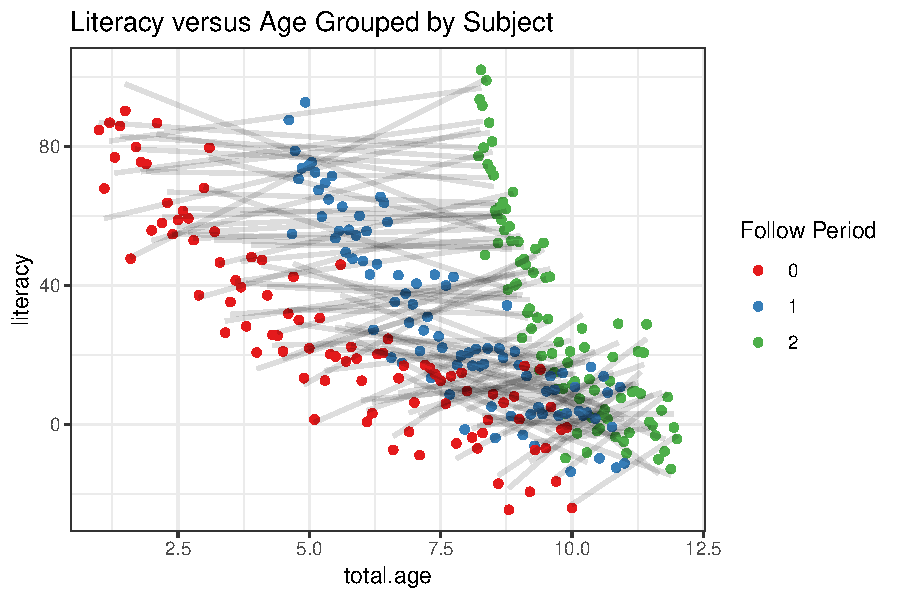
\includegraphics{literacy_versus_age.pdf}
    \caption{Plot of a single realization of the data with $\sigma^2 = 100$. The
      lines are fitted with OLS linear regression conditioned on each subject.}
    \label{fig:literacy_versus_age}
  \end{figure}

  \begin{description}
  \item[Solution:] A single realization is plotted in Figure
    \ref{fig:literacy_versus_age}. By looking at the data from follow period $0$
    and comparing subjects, one can identify the marginal trend: literacy
    decreases with the base age, so younger subjects generally have higher
    literacy. To see the conditional trend, one looks within each subject:
    generally, as a subject ages, their literacy increases. This conditional
    trend isn't very strong, however, since the variance is rather large
    relative to the effect size.
  \end{description}
  
\end{enumerate}
{\em Based on the plot you have generated (and experience from homework 1), it should be clear that
trying to estimate $\beta_L$ by fitting a partitioned model in which you treat $f(x)$ as linear will not work.  
You explain this to your collaborator and propose to fit a model where you include a fixed effect to stratify by
subject.  Your collaborator is sympathetic to the need to deal with confounding but is concerned that fitting a model with $92$ parameters and only $91 \times 3=273$ observations is not a very good idea.  He suggests,
as an alternative, adjusting for subject using a random intercept in a linear mixed effects model (fit using REML, of course).}
\begin{enumerate}[(a)]
\addtocounter{enumi}{1}
\item{\em   Explain to your collaborator, purely in words, why this is a bad idea.}

  \begin{description}
  \item[Solution:] 
  \end{description}
  
\end{enumerate}

{\em Although you're sure that your explanation should have been persuausive, your collaborator is not yet convinced.  So you conduct a simulation to 
further elucidate the differences between estimating $\beta_L$ from models with
fixed effects and random effects for subject-specific intercepts.  }
\begin{enumerate}[(a)]
\addtocounter{enumi}{2}
\item {\em Write down the mathematical form of the two models you will be fitting and describe the simulation study.}


\item {\em  Present and explain the results of your simulation study to your collaborator, highlighting the simulation-based estimates of bias and standard errors of the $\hat{\beta}_L$ you obtain from each model and how these relate to his suggestion.}


\item {\em  Summarize the estimated values of the residual and random effect variances ($\hat{\sigma}^2$ and $\hat{\sigma}^2_\gamma$, respectively) from your simulations.}


\item {\em  Although the subject-specific intercepts in this problem are not really random, there is a natural quantity that you can think of $\hat{\sigma}^2_\gamma$ as trying to estimate.  Calculate this number and call
it $\sigma_\gamma^2$.  Explain how your estimates $\hat{\sigma}^2_\gamma$ compare to  $\sigma_\gamma^2$.}

\end{enumerate}

{\em For the remainder of the problem, consider the idealized situation where REML always estimates the variances
exactly, meaning $\sigma^2=\hat{\sigma}^2=100$ and $\sigma^2_\gamma=\hat{\sigma}^2_\gamma$.}
\begin{enumerate}[(a)]
\addtocounter{enumi}{6}
\item {\em Calculate the exact (to your computer's numerical precision) bias of $\hat{\beta}_L$ from the random effect model as an estimator for $\beta_L$.  Report your answer to five significant digits.  Do this calculation two ways, first by interpreting the estimation procedure as GLS regression and then by interpreting it as penalized OLS regression.   You cannot answer this question with a simulation study, but you are free to use either your own R code or any publicly available R packages for the calculations.  You may find the 
\texttt{penalized} package in R helpful.  Note that although we have seen a theorem that implies these two approaches will give precisely the same answer, in this
problem you are asked to find the solution two separate ways, without using your knowledge that they are equivalent.  }
\item  {\em Using the calculation from part (g) of this problem, plot the bias of $\hat{\beta}_L$ as
a function of $\sigma^2$, over an interesting range of choices for $\sigma^2$ (continue to use the same fixed value
of $\sigma^2_\gamma$ you estimated from the data).}
\item {\em Explain your plot from part (h) of this problem to your collaborator.  Offer two explanations for the pattern in the plot, one based on the clustered WLS (equivalently, GLS) intepretation and the other based on the penalized OLS interpretation of the linear mixed effects model estimation algorithm.}
\item {\em Your collaborator is nearly convinced, but not quite.  He reminds you that you
once told him mixed model effect estimates can be thought of as solutions to a GLS problem and that
any old GLS estimator will do (regardless of correlation structure) to consistently estimate the 
coefficients in a linear regression model.  Explain why this argument doesn't apply in the present situation.}
\end{enumerate}


\end{document}